\documentclass[a4paper, 12pt]{article}
%pack{{{
\usepackage[utf8]{inputenc}
\usepackage[russian]{babel}
\usepackage{amsmath}
\usepackage{graphicx}
\usepackage{listings}
\usepackage{xcolor}
\usepackage{cite}
%}}}
\lstset{ %
language=C++,                % choose the language of the code
basicstyle=\footnotesize,       % the size of the fonts that are used for the code
numbers=left,                   % where to put the line-numbers
numberstyle=\footnotesize,      % the size of the fonts that are used for the line-numbers
stepnumber=1,                   % the step between two line-numbers. If it is 1 each line will be numbered
numbersep=5pt,                  % how far the line-numbers are from the code
backgroundcolor=\color{white},  % choose the background color. You must add \usepackage{color}
showspaces=false,               % show spaces adding particular underscores
showstringspaces=false,         % underline spaces within strings
showtabs=false,                 % show tabs within strings adding particular underscores
frame=single,           % adds a frame around the code
tabsize=2,          % sets default tabsize to 2 spaces
captionpos=b,           % sets the caption-position to bottom
breaklines=true,        % sets automatic line breaking
breakatwhitespace=false,    % sets if automatic breaks should only happen at whitespace
escapeinside={\%*}{*)}          % if you want to add a comment within your code
}
\bibliographystyle{unsrt}
\newcommand{\argmin}{\mathop{\rm arg~min}\limits}
\begin{document}
\tableofcontents
\newpage
\section*{Задание}
\textbf{Решение системы нелинейных уравнений с помощью сочетания
метода наискорейшего спуска и метода Ньютона.}\\
Оценить скорость сходимости метода. На начальном этапе применить
метод наискорейшего спуска, на завершающем – метод Ньютона.
\newpage
\section*{Аннотация}
\addcontentsline{toc}{section}{Аннотация}
В данной работе рассматриваются такие методы нахождения решения систем нелинейных уравнений, как метод простой итерации, методы градиентного и наискорейшего спусков и метод Ньютона.
\newpage
\section*{Введение}
\addcontentsline{toc}{section}{Введение}
Многие задачи физики и математики сводятся к решению систем нелинейных уравнений. При этом, очень часто для решения прикладных задач аналитическое решение не требуется, достаточно вычислить приближенное решение.\\
Для решения систем нелинейных уравнений нет универсального способа решения, поэтому при решении конкретной системы уравнений необходимо
учитывать особенности данных уравнений. Для решения нелинейных систем не существует прямых методов, поэтому импользуются итерационные методы, основанные на существовании стационарной точки у сжимающего оператора, получающегося из системы.\\
Одним из таких методов и является рассматриваемый в данной работе метод Ньютона. Однако, в силу особой чувствительности этого метода
к выбору начального приближения корня, на практике обычно используют более медленный, но менее чувствительный метод наискорейшего спуска
на начальном этапе, получая лучшее приближение для метода Ньютона.
\newpage
\section*{Определения и теоремы}
\addcontentsline{toc}{section}{Определения и теоремы}
\textbf{Функционал} --- традиционное название для функции с областью определения в векторном пространстве и областью значений в множестве действительных чисел\\
\textbf{Норма} --- неотрицательный невырожденный положительно однородный полуаддитивный функционал, определенный на линейном пространстве \\
\textbf{Принцип сжимающих отображений}\\
Пусть $A$ --- отображение полного метрического пространства $(X,\rho_X)$ в себя. Пусть, 
кроме того $\forall x,y \in X$ выполнено следующее неравенство:
\begin{equation}
	\rho (Ax,Ay) \leq q \rho(x,y) \text{,}
\end{equation}
где число $q \in (0,1)$ и не зависит от $x$ и $y$. Тогда существует единственная точка 
$z \in X$ такая, что
\begin{equation}
	Az = z \text{.}
\end{equation}
Такая точка $z$ называется неподвижной.\\
Рассматривая в итерационном процессе $x_n$, как очередное приближение к стационарной точке, можно получить оценку
\begin{equation}
	\rho (x_n,z) \leq \frac{q^n}{1-q} \rho(A(x_0),x_0)
\end{equation}
\nocite{BH}

\newpage
\section*{Описание методов}
\addcontentsline{toc}{section}{Описание методов}
Будем рассматривать систему нелинейных уравнений:
\[
\left\{
\begin{array}{ccc}	f_1(x) & = &  0\\
	f_2(x) & = &  0\\
	\ldots \\
	f_n(x) & = &  0 
\end{array}
\text{,}
\right.
\]
где $x = (x_1, x_2 \ldots x_n)$\\
Общая проблема методов решения систем нелинейных уравнений заключается в их сугубо локальном
характере сходимости. Это сильно затрудняет их применение в случаях, когда имеются проблемы с 
выбором начального приближения.\\
Для решения данной проблемы используют численные методы оптимизации, а именно, минимизации.
Необходимо поставить задачу минимизации таким образом, чтобы её приближенное решение являлось решением 
исходной системы нелинейных уравнений. Для этого, можно, например, ввести функцию:
\begin{equation*}
	\Phi(x) = (f_1(x))^2 + (f_2(x))^2 + \ldots + (f_n(x))^2 \text{,}
\end{equation*}
находя минимум которой, найдем и решение исходной системы. 

\subsection*{Метод градиентного спуска}
Из математического анализа известно, что функция растет быстрее всего в направлении
своего градиента. Значит, оптимальным направлением движения для минимизации будет направление, 
противоположное градиенту в данной точке. То есть, 
для нахождения последующего приближения нужно выбирать точку, смещенную относительно предыдущего
приближения на вектор антиградиента с неким коэффициентом, большим нуля.
\begin{equation}
	x^{(k+1)} = x^{(k)} - \alpha \nabla \Phi(x^{(k)}) \text{,}
\end{equation}
где $\alpha$, вообще говоря, зависит от текущего приближения, то есть $\alpha = \alpha_k$
\subsection*{Метод наискорейшего спуска}
Итак, известно направление, в котором функция убывает быстрее всего. Однако, нужно
еще определить, как далеко в этом направлении нужно искать следующее приближение.
А оптимальным этот шаг будет, если значение $\Phi(x^{(k+1)})$ минимальное из всех возможных в этом направлении.
То есть 
\begin{equation}
	\alpha_k = \argmin_{\alpha > 0} (\Phi(x^{(k)} - \alpha \nabla \Phi(x^{(k)})))
\end{equation}
Сходимость этого метода линейная, что медленнее, чем, скажем, у метода Ньютона. Однако, как
говорилось выше, метод Ньютона, как и другие, чувствителен к выбору начального приближения.
Используя на начальном этапе метод наискорейшего спуска можно найти хорошее приближение для него.\\
Немного о реализации $argmin$. Использовать будем троичный поиск. Выбранный интервал разбивается на три равных интервала.
Пусть, скажем, изначальный интервал был $[a,b]$. Тогда выбираются точки $m_1 = a+\frac{b-a}{3}$ и $m_2 = b-\frac{b-a}{3}$ и сравниваются значения в них.
Допустим, ищется минимум. Если $f(m_1) > f(m_2)$, то $a = m_1$, в противном случае $b = m_2$. Алгоритм запускается заново с новыми параметрами.
Так продолжается до тех пор, пока $||a - b|| > \epsilon$, где $\epsilon$ --- один из параметров алгоритма --- наименьшая длина отрезка, на котором ищется минимум,при достижении которой поиск останавливается и выбирается точка посередине такого отрезка. В итоге, можно достигнуть точности
\begin{equation*}
	||\argmin_{\alpha}(f(\alpha)) - \frac{a+b}{2})|| \leq \frac{\epsilon}{2}.
\end{equation*}

\subsection*{Метод Ньютона}
Если определено начальное приближение $x^{(0)}$, итерационный процесс нахождения решения системы методом Ньютона можно представить в виде 
\begin{equation}
	x^{(k+1)} = x^{(k)} + \Delta x^{(k)}\text{,}
\end{equation}

где значения $\Delta x^{(k)}$ определяются из решения системы линейных алгебраических уравнений, все коэффициенты которой выражаются
через известное предыдущее приближение $x^{(k)}$. Вектор приращений
\begin{equation*}
	\Delta x^{(k)} = 
	\left(
	\begin{tabular}{c}
		$ \Delta x^{(k)}_1$\\ 
		$ \Delta x^{(k)}_2$\\ 
		$ \Delta x^{(k)}_3$\\ 
		$ \ldots         $ \\ 
		$ \Delta x^{(k)}_n$
	\end{tabular}
	\right)
\end{equation*}
находится из решения уравнения
\begin{equation}
	f(x^{(k)}) + J(x^{(k)}) \Delta x^{(k)} = 0 \text{.}
\end{equation}
Здесь \[J = \left(
	\begin{tabular}{cccc}
		$\frac{\partial f_1(x)}{\partial x_1}$&$\frac{\partial f_1(x)}{\partial x_2}$&$\ldots$&$\frac{\partial f_1(x)}{\partial x_n}$\\
		$\frac{\partial f_1(x)}{\partial x_1}$&$\frac{\partial f_2(x)}{\partial x_2}$&$\ldots$&$\frac{\partial f_2(x)}{\partial x_n}$\\
		$\ldots$&$\ldots$&$\ldots$&$\ldots$\\
		$\frac{\partial f_n(x)}{\partial x_1}$&$\frac{\partial f_n(x)}{\partial x_2}$&$\ldots$&$\frac{\partial f_n(x)}{\partial x_n}$
	\end{tabular}\\
\right) \text{--- Матрица Якоби }\] первых производных вектор-функции $f(x)$.
Выражая из $(7)$ вектор приращений $\Delta x^{(k)}$ и подставляя его в $(6)$, итерационный процесс нахождения решения можно записать в виде 
\begin{equation}
	x^{(k+1)} = x^{(k)} + [J(x^{(k)})]^{-1} f(x^{(k)})\text{.}
\end{equation}
При реализации алгоритма метода Ньютона в большинстве случаев предпочтительным является не вычисление обратной матрицы Якоби, а нахождение 
из системы (7) значений приращений $\Delta x^{(k)}$ и вычисление нового приближения по (6).\\
Использование метода Ньютона предполагает дифференцируемость функций $f_1(x),\ldots ,f_n(x)$ и невырожденность матрицы Якоби. В случае, если 
начальное приближение выбрано в достаточно малой окрестности искомого корня, итерации сходятся к точному решению, причем сходимость квадратичная(если только якобиан в точке решения не равен или близок к нулю).\\
В практических вычислениях в качестве условия окончания итераций обычно используется критерий 
\begin{equation}
	|| x^{(k+1)} - x^{(k)} || \leq \epsilon \text{,}
\end{equation}
где $\epsilon$ --- заданная точность.
\newpage
\section*{Листинг программы}
\addcontentsline{toc}{section}{Листинг программы}
\lstinputlisting{main.cpp}

\newpage
\section*{Пример работы}
\addcontentsline{toc}{section}{Пример работы}
Для примера будет использоваться система из двух нелинейных уравнений 
\begin{equation}
	\left\{
		\begin{tabular}{cc}
			$x^2 + y^2 - 1 $&$ = 0$\\
			$x-y+0.5$&$ = 0$
		\end{tabular}
		\right.
\end{equation}
Решением которой с точностью до $10^{-7}$ является $(0.411438, 0.911438)$. Существует еще одно решение, вторая точка пересения прямой и окружности. Его мы
здесь рассматривать не будем.\\
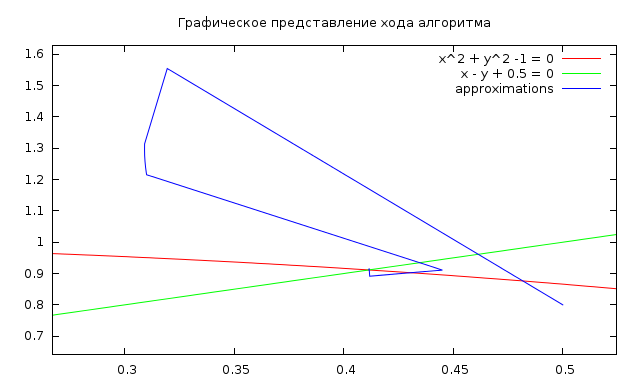
\includegraphics[width=\linewidth]{xs.png}
	\begin{center}
		рис. 1\\
	\end{center}
\subsection*{Зависимости количества итераций от начальных приближений и точности}
\vfil
	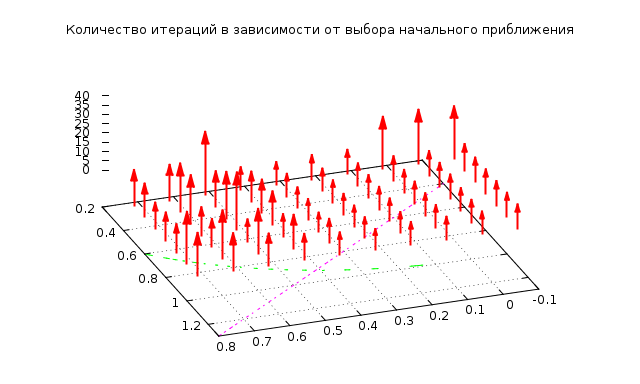
\includegraphics[width=\linewidth]{p0.png}\\
	\begin{center}
		рис. 2\\
	\end{center}
\vfil
	На рисунке 2 явно просматривается тенденция увеличения количества итераций при удалении от точки решения.\\
\newpage
\vfil
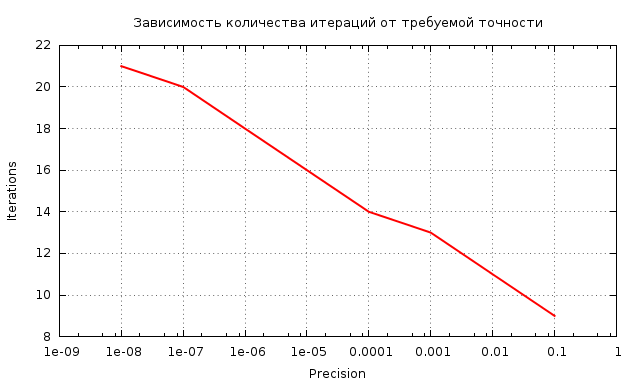
\includegraphics[width=\linewidth]{eps.png}
	\begin{center}
		рис. 3\\
	\end{center}
\vfil
На рисунке 3 изображено суммарное количество итераций (сначала методом наискорейшего спуска, потом и методом Ньютона). При этом для метода наискорейшего спуска была
задана фиксированная точность $0.01$, а для метода Ньютона значения, которые можно выделены на оси абсцисс. Из графика на этом рисунке можно сделать вывод, что существенное увеличение точности
не влечет большого роста количества итераций в методе Ньютона при хорошем начальном приближении.
\newpage
\section*{Заключение}
\addcontentsline{toc}{section}{Заключение}
В результате выполнения работы были достигнуты следующие результаты:\\
\begin{itemize}
	\item Написана программа, решающая системы нелинейных уравнений различной размерности, в пространствах с разными нормами с задаваемой точностью
	\item Исследована скорость сходимости связки методов при различных входных данных и точности
\end{itemize}
\newpage
\addcontentsline{toc}{section}{Список литературы}
\nocite{nm_verg_a}
\nocite{nm_verg_m}
\nocite{RH}
\nocite{RS}
\bibliography{article}

\end{document}
